\fancyhf{}
\fancyhead[C]{\textbf{КВАНТ \hspace{1mm} 2012 / № 5--6}}
\fancyhead[R]{}

\singlespacing
\setlist{itemsep=2pt, topsep=0pt, parsep=-2.3pt, partopsep=0pt}
% \titlespacing*{\subsection}{0pt}{14pt}{\baselineskip}
\titlespacing*{\section}{0pt}{-5pt}{\baselineskip}
\setlength{\leftmargini}{12pt}
\setlength{\tabcolsep}{6pt}
\setlength{\intextsep}{15pt}
\fontsize{8}{12}\selectfont
\fancyhead[L]{69}
\vspace*{\fill}
\section*{\centering LIII Международная математическая олимпиада}
\begin{multicols}{2}
    {\par \hspace*{0.2cm}С 4 по 16 июля 2012 года в Аргентине прошла LIII Международная математическая олимпиада (ММО). Прохладной аргентинской зимой олимпиаду принимал курортный город Мар-дель-Плата, расположенный на берегу Атлантического океана. В этом году в ММО приняли участие 548 человек из 100 стран мира.}
    {\par \hspace*{0.2cm}Команду России составили ребята из самых разных уголков нашей страны: выпускники школы Михаил Григорьев из Казани (лицей 131) и Александр Калмынин из Иркутска (лицей-интернат 1), десятиклассники Дмитрий Крачун из Санкт-Петербурга (ФМЛ 239), Александр Матушкин из Ижевска (лицей 29), Лев Шабанов из Ангарска Иркутской области (СУНЦ МГУ) и девятиклассник Даниил Клюев из Санкт-Петербурга (ФМЛ 239). Несмотря на то, что сборная России нынешнего года достаточно молодая (большая часть команды имеет шансы и на следующий год принять участие в ММО), каждый из ребят в рамках подготовки сборной к ММО уже участвовал хотя бы в одном из международных соревнований, а Михаил Григорьев и Дмитрий Крачун завоевали медали ММО в прошлом году. Задания нынешней олимпиады оказались весьма сложными (только 32 участника (!) сумели набрать более двух третей от возможного максимального числа баллов), особенно трудными были задачи 3 и 6. Тем не менее, наша сборная выступила успешно. Российские школьники завоевали 4 золотые и 2 серебряные медали, заняв 4 строчку в командном рейтинге.}
    {\par \hspace*{0.2cm}Последний этап подготовки команды к ММО – летние учебно-тренировочные сборы – проходил, как и в предыдущие годы, в детском лагере «КОМПЬЮТЕРиЯ» (Тверская область). Большой вклад в успешное выступление команды внесли преподаватели сборов: педагог ФМЛ 239 Санкт-}
    \newcolumn
    \columnbreak
    \begin{figure}[H]
        \centering
        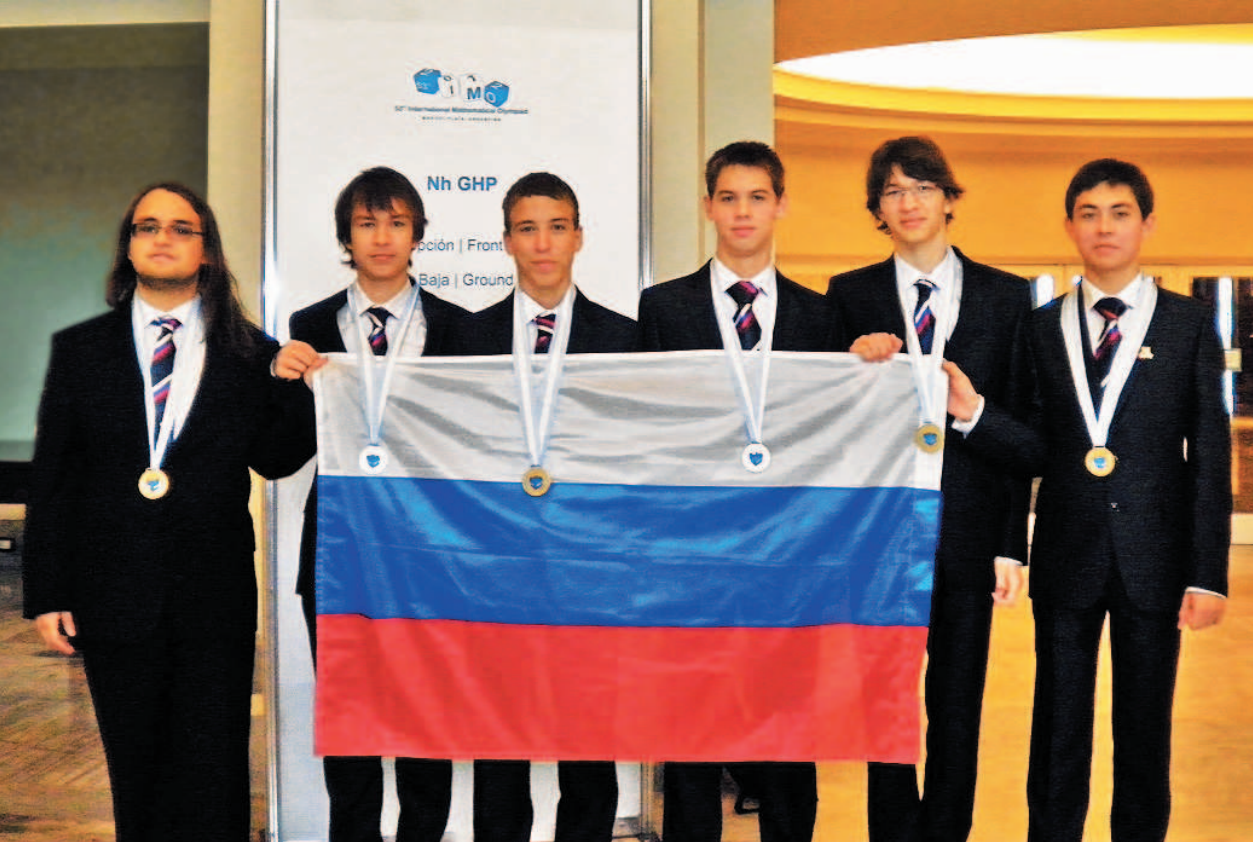
\includegraphics[width=0.5\textwidth]{pic.png}
        \captionsetup{font=scriptsize,labelformat=empty}
        \caption{\textit{Слева направо: А.Калмынин, Л.Шабанов, Д.Крачун, А.Матушкин, Д.Клюев, М.Григорьев}}
    \end{figure}
    \vspace{-\baselineskip}
    {\par \hspace*{0.2cm}Петербурга, к.ф.-м.н. С.Л.Берлов, младший научный сотрудник, преподаватель МГУ и МФТИ, к.ф.-м.н. А.И.Гарбер, педагог дополнительного образования Санкт-Петербурга А.С.Голованов, профессор Ярославского государственного университета, д.ф.-м.н. В.Л.Дольников, аспирант МГУ А.Н.Магазинов, аспирант МГУ И.Митрофанов, аспирант СПбГУ К.А.Сухов, аспирант ЯрГУ Г.Р.Челноков}
    {\par \hspace*{0.2cm}Приводим результаты выступления нашей сборной (каждая задача оценивалась из 7 баллов). Полная информация о результатах на международных математических олимпиадах имеется на официальном сайте олимпиады www.imo-official.com}
\end{multicols}
\newpage
\fancyhead[L]{70} % Левый верхний угол
\begin{multicols}{2}
    {\par \hspace*{-0.9cm}
    \begin{tabular}{c c c c c c c c c}
        Участник & \multicolumn{6}{c}{Баллы по задачам} & Сумма & Медаль \\ 
        & 1 & 2 & 3 & 4 & 5 & 6 & & \\ 
        \makecell[{{p{1.5cm}}}]{\raggedright Григорьев\\Михаил} & 7 & 7 & 5 & 7 & 7 & 0 & 33 & золотая \\ 
        \makecell[{{p{1.5cm}}}]{\raggedright Кальмынин\\Александр} & 7 & 7 & 0 & 7 & 7 & 0 & 28 & золотая \\ 
        \makecell[{{p{1.5cm}}}]{\raggedright Клоев\\Даниил} & 7 & 7 & 7 & 7 & 7 & 0 & 35 & золотая \\ 
        \makecell[{{p{1.5cm}}}]{\raggedright Крачун\\Дмитрий} & 7 & 7 & 3 & 7 & 7 & 1 & 32 & золотая \\ 
        \makecell[{{p{1.5cm}}}]{\raggedright Матушкин\\Александр} & 7 & 7 & 3 & 7 & 1 & 1 & 26 & серебряная \\ 
        \makecell[{{p{1.5cm}}}]{\raggedright Шабанов\\Лев} & 7 & 0 & 3 & 6 & 0 & 7 & 23 & серебряная \\ 
    \end{tabular}
    }
    {\par \hspace*{0.2cm}Руководители команды благодарят Д.Ю.Дойхена, который много лет оказывает поддержку команде России в международных математических соревнованиях. }
    \subsection*{\centering\scriptsize ЗАДАЧИ ОЛИМПИАДЫ}
    \begin{enumerate}
        \item Дан треугольник \textit{ABC}; точка \textit{J} является центром вневписанной окружности, соответствующей вершине \textit{A}. Эта вневписанная окружность касается отрезка \textit{BC} в точке \textit{M}, а прямых \textit{A}B и \textit{AC} – в точках \textit{K} и \textit{L} соответственно. Прямые \textit{LM} и \textit{BJ} пересекаются в точке \textit{F}, а прямые \textit{KM} и \textit{CJ} пересекаются в точке \textit{G}. Пусть \textit{S} – точка пересечения прямых \textit{AF} и \textit{BC}, а \textit{T} – точка пересечения прямых \textit{AG} и \textit{BC}. Докажите, что точка \textit{M} является серединой отрезка \textit{ST}. \par\hfill \textit{Греция}
        \item Дано целое число $\textit{n} \geq 3$ и действительные положительные числа $a_2, a_3, \dots, a_n$ такие, что $a_2 a_3 \dots a_n = 1$. Докажите, что
            \begin{equation*}
                    (1 + a_2)^2 (1 + a_3)^3 \dots (1 + a_n)^n > n^n
            \end{equation*}
                \par\hfill \textit{Австралия}
        \item Два игрока \textit{A} и \textit{B} играют в игру «Угадай-ка». Правила этой игры зависят от двух положительных целых чисел \textit{k} и \textit{n}, и эти числа известны обоим игрокам. \\ В начале игры \textit{A} выбирает целые числа \textit{x} и \textit{N} такие, что $1 \leq x \leq N$. Игрок \textit{A} держит число \textit{x} в секрете, а число \textit{N} честно сообщает игроку \textit{B}. После этого игрок \textit{B} пытается получить информацию о числе \textit{x}, задавая игроку \textit{A} вопросы следующего типа: за один вопрос \textit{B} указывает по своему
    \columnbreak
        усмотрению множество \textit{S}, состоящее из целых положительных чисел (возможно, это множество уже было указано в одном из предыдущих вопросов), и спрашивает игрока \textit{A}, принадлежит ли число \textit{x} множеству \textit{S}. Игрок \textit{B} может задать столько вопросов, сколько он хочет. На каждый вопрос игрока \textit{B} игрок \textit{A} должен сразу ответить «да» или «нет», при этом ему разрешается соврать столько раз, сколько он хочет; единственное ограничение состоит в том, что из любых \textit{k} + 1 подряд идущих ответов хотя бы один ответ должен быть правдивым. \\ После того как \textit{B} задаст столько вопросов, сколько он сочтет нужным, он должен указать множество \textit{X}, содержащее не более \textit{n} целых положительных чисел. Если \textit{x} принадлежит множеству \textit{X}, то игрок \textit{B} выиграл; иначе \textit{B} проиграл. Докажите, что:
        \begin{enumerate}
            \item Если $n \geq 2^k$, то \textit{B} может гарантировать себе выигрыш.
            \item Для всякого достаточно большого \textit{k} найдется целое число $n \geq 1,99^k$, при котором игрок \textit{B} не сможет гарантировать себе выигрыш. \par\hfill \textit{Канада}
        \end{enumerate}
        \item Найдите все функции $f: \mathbb{Z} \to \mathbb{Z}$ такие, что для любых целых чисел $a, b, c$, удовлетворяющих условию $a + b + c = 0$, выполняется равенство
            \begin{equation*}
                f(a)^2+f(b)^2+f(c)^2=2f(a)f(b)+2f(b)f(c)+2f(c)f(a)
            \end{equation*}
            \par\hfill \textit{Южная Африка}
        \item Пусть \textit{ABC} – треугольник, в котором $\angle BCA = 90^\circ$ , и пусть \textit{D} – основание высоты, проведенной из вершины \textit{C}. Внутри отрезка \textit{CD} взята точка \textit{X}. Пусть \textit{K} – точка, лежащая на отрезке \textit{AX} такая, что $BK = BC$. Аналогично, пусть \textit{L} – точка, лежащая на отрезке \textit{BX} такая, что $AL = AC$. Пусть \textit{M} – точка пересечения отрезков \textit{AL} и \textit{BK}. Докажите, что $MK = ML$.\par\hfill \textit{Чехия}
        \item Найдите все целые положительные числа \textit{n}, для которых существуют целые неотрицательные числа $a_1, a_2, ..., a_n$ такие, что
            \begin{equation*}
                \frac{1}{2^{a_1}} + \frac{1}{2^{a_2}} + ... + \frac{1}{2^{a_n}} = \frac{1}{3^{a_1}} + \frac{1}{3^{a_2}} + ... + \frac{n}{2^{a_n}} = 1
            \end{equation*}
            \par\hfill \textit{Сербия}
            \par\raggedleft \textit{Публикацию подготовили Н.Агаханов, И.Богданов, П.Кожевников, М.Пратусевич, Д.Терёшин}
    \end{enumerate}
    \end{multicols}
\section*{\centering XLIII Международная физическая олимпиада}
\begin{multicols}{2}
    {\par\hspace*{0.2cm}В 2012 году Международная олимпиада школьников по физике (IPhO) проходила в Эстонии с 15 по 23 июля. В олимпиаде приняли участие школьники из 81 страны. }
    {\par\hspace*{0.2cm}Россию на олимпиаде представляли \textit{Никита Сопенко (Тамбовская область), Лев Гинзбург (Хабаровск), Иван Ивашковский (Москва), Александра Васильева (Москва) и Давид Френклах (Долгопрудный Московской обл.). }}
    {\par\hspace*{0.2cm}Эти ребята прошли долгий путь отбора и подготовки к Международной олимпиаде. В апреле 2011 года по результатам заключительного этапа Всероссийской олимпиады по физике 2011 года были отобраны 24 десятиклассника, которые стали кандидатами в Национальную сборную России. }
    {\par\hspace*{0.2cm}Для них были проведены три двухнедельных сбора, во время которых с ребятами занимались ведущие преподаватели физики МФТИ, научные сотрудники ИТЭФ, ЦАГИ. По результатам сборов, а также с учетом результатов заключительного этапа Всероссийской олимпиады школьников по физике 2012 года были отобраны пятеро ребят, которые и поехали на олимпиаду. }
    {\par\hspace*{0.2cm}Важным элементами подготовки сборной стало участие наших кандидатов в Европейской олимпиаде по физике в Румынии (Бухарест, март 2012 г.) и в Азиатской олимпиаде школьников по физике (Нью-Дели, май 2012 г.). На обеих олимпиадах наши ребята выступили достаточно успешно. В }
\end{multicols}
